% LaTex file for Stephen Balakirsky's RITA 2014 submission
%
\documentclass{llncs}
%
\usepackage{makeidx}  % allows for indexgeneration
%
% my additional packages
\usepackage{graphicx}
%\usepackage{multirow,array}
%\usepackage{rotating} % for sideways
\usepackage{amsmath}
\usepackage{fancyvrb}
\usepackage{subfigure}
\usepackage{tikz}
%\usepackage{algorithm2e}
\usepackage[linesnumbered, boxed, figure]{algorithm2e}
%
% zeid's definitions
\newcommand{\class}[1] {\textit{#1}}
\newcommand{\const}[1] {$\mathit{#1}$}
\newcommand{\objvar}[1] {$\mathsf{#1}$}
\newcommand{\stvar}[1] {\textsf{#1}}
\newcommand{\constsmall}[1] {\small $\mathit{#1}$}
\newcommand{\stvarsmall}[1] {\small {\textsf{#1}}}
\newcommand{\op}[1] {\textsl{#1}}
\newcommand{\opsmall}[1] {\small {\textsl{#1}}}
\newcommand{\nil} {\textit{nil}\ }
\newcommand{\app}[1] {\textit{#1}}
\newcommand{\file}[1] {\textsf{#1}}
\newcommand*\mycirc[1]{%
  \begin{tikzpicture}
    \node[draw,circle,inner sep=0.5pt] {#1};
  \end{tikzpicture}}
%
%
\begin{document}
%
\frontmatter          % for the preliminaries
%
\pagestyle{headings}  % switches on printing of running heads
\addtocmark{Hamiltonian Mechanics} % additional mark in the TOC
%
%
\mainmatter              % start of the contributions
%
%\title{Development of a Canonical Sensor Command/Response Language for Industrial Kit Building Applications}
\title{A Simulated Sensor-based Approach for Kit Building Applications}
%
\titlerunning{Agile Manufacturing}  % abbreviated title (for running head)
%                                     also used for the TOC unless
%                                     \toctitle is used
%
\author{Zeid Kootbally\inst{1}, Craig Schlenoff\inst{2}, Teddy Weisman\inst{3}, Stephen Balakirsky\inst{4}, Thomas Kramer\inst{5}, and Anthony Pietromartire\inst{2}}

%
\authorrunning{Zeid Kootbally et al.} % abbreviated author list (for running head)
%
%%%% list of authors for the TOC (use if author list has to be modified)
\tocauthor{Zeid Kootbally, Craig Schlenoff, Teddy Weisman, Stephen Balakirsky, and Anthony Pietromartire}
%
\institute{
University of Maryland, College Park, MD 20740, USA,\\
\email{zeid.kootbally@nist.gov},\\ WWW home page:
\texttt{www.nist.gov/el/isd/ks/kootbally.cfm}
\and
Intelligent Systems Division, National Institute of Standards and Technology, Gaithersburg, MD, USA,\\
\email{craig.schlenoff@nist.gov, anthony.pietromartire@nist.gov},\\
WWW home page:
\texttt{www.nist.gov/el/smartcyber.cfm}
\and
Yale University, New Haven, CT 06520,\\
\email{tjweisman@gmail.com}
\and
Georgia Tech Research Institute, Atlanta, GA 30332, USA,\\
\email{stephen.balakirsky@gtri.gatech.edu},\\
WWW home page:
\texttt{unmannedsystems.gtri.gatech.edu}
\and
Department of Mechanical Engineering, Catholic University of America, Washington, DC, USA,\\
\email{thomas.kramer@nist.gov},\\
WWW home page:
\texttt{http://www.nist.gov/el/isd/ks/kramer.cfm}
}

\maketitle              % typeset the title of the contribution



%
% ---- Sections ----
%
%---------------------------%
\begin{abstract}
Kit building or kitting is a process in which separate but related items are grouped, packaged, and supplied together as one unit (kit). 
This paper describes advances in the development of kitting simulation tools that incorporate sensing/control and parts detection capabilities. To pick 
and place parts and components during kitting, the kitting workcell relies on a simulated sensor system to retrieve the six-degree of freedom (6DOF) pose estimation of each of these objects. While the use of a sensor system allows objects' poses to be obtained, it also helps detecting failures during the execution of a kitting plan when some of these objects are missing or are not at the expected locations. A simulated kitting system is presented and the approach that is used to task a sensor system to retrieve 6DOF pose estimation of specific objects (objects of interest) is given.
\end{abstract}
\keywords{simulation, manufacturing, robotics, kitting, sensor system} 
%---------------------------%
\section{Introduction}
\section{Introduction}
A failure is any change, design, or manufacturing error that renders a component, assembly, or system incapable of performing its intended function \cite{Collins93}. In kitting, as described in Section \ref{sect:kitting}, failures can occur for multiple reasons that include equipment not being set up properly, tools and/or fixtures not being properly prepared, and improper equipment maintenance. Part/component availability failures can be triggered by inaccurate information on the location of the part, part damage, incorrect part types, or part shortage due to delays in internal logistics. In order to prevent or minimize failures, a disciplined approach needs to be implemented to identify the different ways a process design can fail before impacting productivity.

Even though today's state-of-the-art industrial robots are capable of sub-millimeter accuracy \cite{RobotAccuracy}, they often lack the sensing
necessary to detect failures and the programming required to cope with and correct the failure. This is due to the fact that they are often programmed
by an operator using crude positional controls from a teach pendant. These teach pendant programs are highly repeatable, which provides 
utility for large-batch, error-free operation. However, the cyclic program that repeats identical operations does not lend itself well to adaptation for 
failure mitigation. In fact, producing a program to correct a perceived failure would require that the cell be taken off-line
for additional human-led teach pendant programming. In addition, 
most cells lack the ability to sense that a failure occurred and  lack programming (that would have had to be teach pendant entered) to cope
with failure conditions, thus making it impossible for the cell to recover from failures.
This leads to faulty products being sent down the line, and/or downtime for the cell as failures are detected and corrected.

For small batch processors or other customers who must frequently change their line configuration or desire to perform complex operations
with their robots, this frequent downtime and lack of failure correction/detection may be unacceptable. The robotic systems of tomorrow need to be capable, flexible, and agile.  
These systems need to perform their duties at least  as well as human counterparts, be quickly re-tasked to other operations, cope with a wide 
variety of unexpected environmental and operational changes, and be able to detect and correct errors in operation. 
To be successful, these systems need to combine domain expertise, knowledge of their own skills and limitations, and both semantic and geometric 
environmental information.

The IEEE Robotics and Automation Society's Ontologies for Robotics and Automation Working Group has taken the first steps in creating the 
infrastructure necessary for such a system, while the Industrial Subgroup has applied this infrastructure to create a sample kit building
system.  This work is presented in Balakirsky et al. \cite{balakirsky2013} which describes the construction of a robotic kit building
system that is able to cope with environmental and task changes without operator intervention. This article extends that work to utilize
the same infrastructure to allow for the detection and correction of action failures in the system.

The organization of the remainder of this paper is as follows. Section \ref{sect:kitting} describes the domain of kit building. Section \ref{sect:overview} presents
an overview of the software system architecture as well as details of the ontology and world model for the robot cell. Section \ref{sect:operation} discusses the detailed operation of cell, and Section \ref{sect:failure} discusses how failures are handled by the ontology. Finally, Section \ref{sect:future} presents
conclusions and future work.
%
%
\section{Kitting}
\label{sect:kitting}
Today's advanced manufacturing plants utilize mixed-model assembly where multiple product variants are built on the same line.  
According to Jim Tetreault, Ford’s vice president of North America Manufacturing, 
new Ford assembly facilities are able to build a full spectrum of vehicles on the same assembly line \cite{James2011}. One of the technologies that makes this possible
is the use of assembly kits.  Bozer and McGinnis \cite{Bozer1992} describe a kit as ``a specific
collection of components and/or subassemblies that together (i.e., in the same container) support one or more assembly
operations for a given product or shop order''. These  kits provide a synchronous material flow, where parts and components move to 
assembly stations in a just-in-time manner. The kits provide workers with the parts and tools that they need (which may vary from 
vehicle model to vehicle model) in the sequence that they need them. The use of kitting also allows a single delivery system to feed
multiple assembly stations thus saving manufacturing or assembly space \cite{Medbo2003} and provides an additional inspection opportunity 
that allows for the detection of part defects before they impact assembly operations. The individual operations of the station 
that builds the kits may be viewed as a specialization of the general
bin-picking problem \cite{Schyja2012} where parts are picked from one or more part bins or trays and placed into specific slots in a kit tray.

For our sample implementation, we assume that the robot cell is building one of several possible kit configurations. At execution time, the
cell has a set kit to build, but does not know the precise location of the kit tray, the part trays, or the location of individual parts in the part tray.
When a human builds a kit, they are able to inspect each part before adding it to the kit tray. This provides an additional level of quality control and
is an aspect that is desirable to have in our robotic system. During kit construction,
a robot performs a series of pick-and-place operations
in order to construct the kit. These operations include:
\begin{enumerate}
\item Pick up an empty kit and place it on the work table.
\item Pick up multiple component parts, inspect them, and place them in the kit.
\item Pick up the completed kit and place it in the full kit storage area.
\end{enumerate}
Each of these steps may be a compound action that includes
other actions such as end-of-arm tool changes, path planning,
and obstacle avoidance. The items that are being placed in the kit may be of varying size and shape and have various grasping and inspection
requirements.
%
\begin{figure}[htb!]
\begin{center}
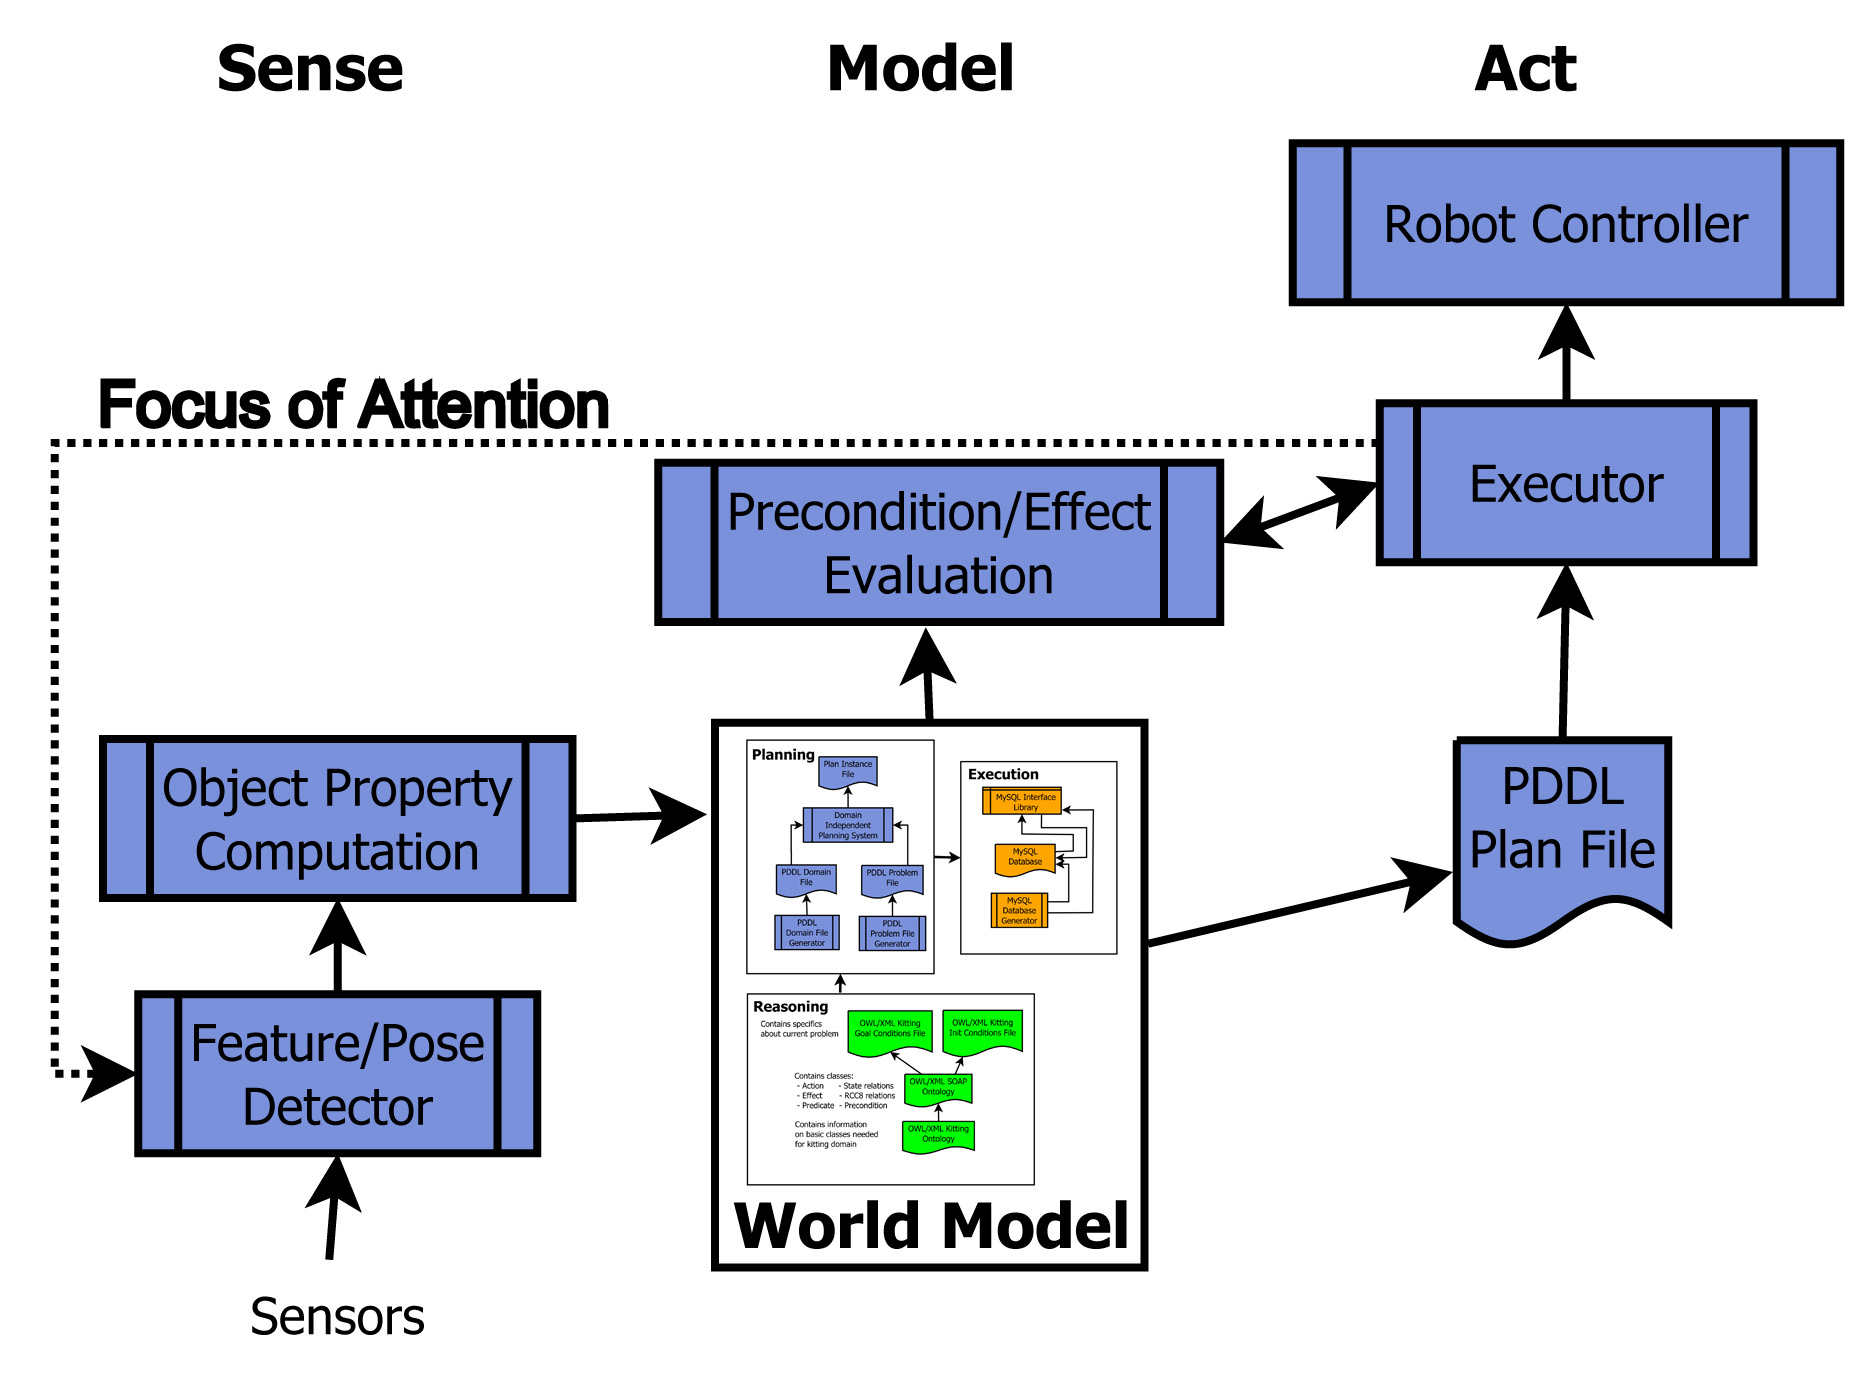
\includegraphics[width=8.5cm]{images/RITAExecution.jpg}
\caption{Major components that make up the Sense--Model--Act paradigm of the kitting station.}
\label{fig:SenseModelAct}
\end{center}
\end{figure}
%---------------------------%
\section{Knowledge Driven Methodology}\label{section:architecture}
\begin{figure}[!t!h!b!]
\centering
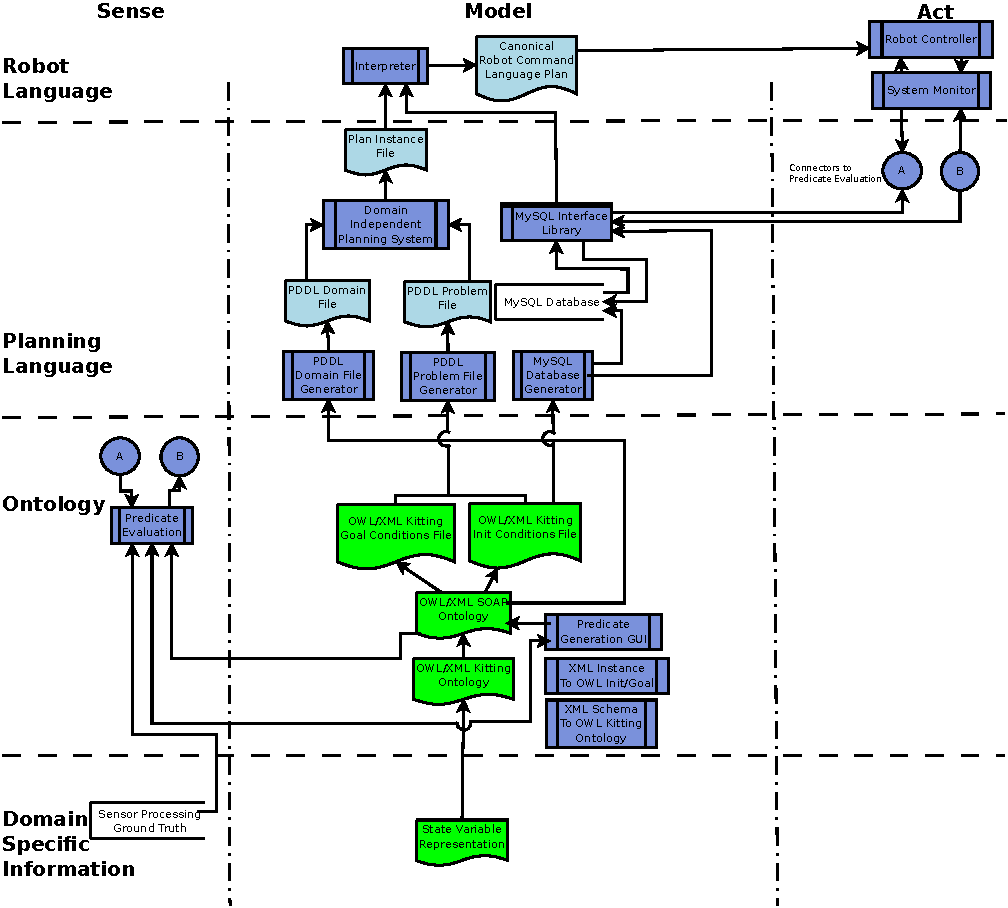
\includegraphics[width=12cm]{images/KnowledgeDrivenRobotics.pdf}
\caption{Knowledge Driven Design extensions -- In this figure, green shaded
  boxes with curved bottoms represent hand generated files while light blue
  shaded boxes with curved bottoms represent automatically created boxes.
  Rectangular boxes represent processes and libraries. }
\label{fig:methodology}
\end{figure}


The knowledge driven methodology presented in this section is not intended to act as a stand-alone system architecture. Rather it is intended to be an extension to well-developed hierarchical, deliberative architectures such as 4D/RCS (Real-time Control Systems)~\cite{Albus2000}. The overall knowledge driven methodology of the system is depicted in Figure~\ref{fig:methodology}. The figure is organized vertically by the representation that is used for the knowledge and horizontally by the classical sense-model-act paradigm of intelligent systems. The remainder of this section gives a brief description of each level of the hierarchy to help the reader understand the basic concepts implemented within the system architecture in order that the reader may better grasp the main effort described in this paper. The reader may find a more detailed description of each component and each level of the architecture in other publications~\cite{BALAKIRSKY.IROS.2012}.

\subsection{Domain Specific Information}
\label{subsection:DSI}
On the vertical axis, knowledge begins with Domain Specific Information (DSI). DSI includes sensors and sensor processing that are specifically tuned to operate in the target domain. Examples of sensor processing may include pose determination and object identification. It is important to note that the effort described in this paper assumes perfect data from the sensor system that do not include noise. A detailed description of the simulated sensor system is given in Section~\ref{sect:simulation}.

For the knowledge model, a scenario driven approach is taken where the DSI design begins with a domain expert creating one or more use cases and specific scenarios that describe the typical operation of the system. This includes information on items ranging from what actions and attributes are relevant, to what the necessary conditions (preconditions) are for an action to occur and what the likely results (effects) of the action are. The authors have chosen to encode this basic information in a formalism known as a state variable representation~\cite{NAU.2004}.


\subsection{Ontology}
\label{subsection:ontology}
The information encoded in the DSI is then organized into a domain
independent representation.

\begin{itemize}
\item A Web Ontology Language (OWL)/Extensible Markup Language (XML) base ontology (\textsf{OWL/XML Kitting})
contains all of the basic information that was determined to be needed
during the evaluation of the use cases and scenarios. The knowledge is
represented in a compact form with knowledge classes
inheriting common attributes from parent classes.
\item The \textsf{OWL/XML SOAP} ontology describes the links between States, Ordering constructs, Actions, and Predicates (the SOAP
ontology) that are relevant to the scenario. A State is composed of one to many state relationships, which is
a specific relation between two objects (e.g., Object 1 is on top of Object 2). An Ordering construct defines the order in which the state relationships need to be
represented for a specific State. In classical representation, States are represented as sets of logical
atoms (Predicates) that are true or false within some interpretation. Actions are represented by
planning operators that change the truth values of these atoms. In the case of the kit building domain, it was found that 10 actions and
16 predicates were necessary.

\item The instance files describe the initial and goal states for the
system through the \textsf{Kitting Init Conditions File} and the
\textsf{Kitting Goal Conditions File}, respectively. The initial state file
must contain a description of the environment that is complete enough for a
planning system to be able to create a valid sequence of actions that will
achieve the given goal state. The goal state file only needs to contain
information that is relevant to the end goal of the system. For the case of building a kit, this may simply be that a complete kit is located in a bin designed to hold completed kits.

\end{itemize}




%The \textsf{OWL/XML SOAP} ontology describes not only aspects of actions and predicates but also the
%individual actions and predicates that are necessary for the domain under study.



%
% <<<<<<< HEAD
% Since both the OWL (Web Ontology Language) \cite{OWLoverview} and XML implementations of the knowledge representation are file based, real-time information proved to be problematic. In order to solve this problem, an automatically generated MySQL database has been introduced as part of the knowledge representation.
% While the knowledge representation presented in this paper provides the \lq\lq{}slots\rq\rq{} necessary for representing dynamic information, the
% static file structure makes the utilization of these slots awkward. It is desirable to be able to represent the dynamic information in a dynamic database. For this reason, the authors have developed a technique for automatically generating tables for storing,  and access functions for obtaining, the data from the ontology in a MySQL database.
%
% Reading data from and to the MySQL database instead of the ontology file offers the community easy access to a live data structure. Furthermore, it is more practical to modify the information stored in a database than if it was stored in an ontology, which in some cases, requires the deletion and re-creation of the whole file. A literature review reveals many efforts and methodologies that have been designed to produce SQL databases from ontologies. Our effort builds upon the work of Astrova et al.\cite{Astrova2007}.
%
% In addition to generating and filling the database tables, the authors have created tools that automatically generate a set of C{}\texttt{++} classes for reading and writing
% information to the kitting MySQL database. The choice of C{}\texttt{++} was a team preference and we believe that other object-oriented languages could have been used in this project.
%
% The interaction of the MySQL database with the Connectors to Predicate Evaluation (in the Act level) is detailed in Section \ref{sec:sensor-1}.
%
% =======
Since both the OWL and XML implementations of the knowledge representation are file-based, real time information proved to be problematic. In order to solve this problem, an automatically generated \textsf{MySQL Database} \cite{MySQL} was introduced as part of the knowledge representation. A description of the \textsf{MySQL Database} is given in the following subsection.


%
%The Generator tool is a graphical user interface developed in Java, allowing the user to store data from OWL files into a MySQL database. This tool also permits the user to query the database using the C++ function calls. The tool Generator is composed of the following functionalities:
%\begin{enumerate}
% \item Convert OWL documents into SQL syntax (OWL to SQL).
% \item Translate SQL syntax to OWL language in order to modify an OWL document (SQL to OWL).
% \item Convert the OWL language into C++ classes (OWL to C++).
%\end{enumerate}
%
%To date, only steps 1. and 3. have been implemented and will be covered in this document.
%In order to generate the SQL database and C++ classes, the OWL object model must be mapped to the C++ object model and the relational SQL model.
%To quote the OWL 2 Web Ontology website~\cite{OWLspec}, ``Entities are the fundamental building blocks of OWL 2 ontologies,
%and they define the vocabulary --the named terms-- of an ontology. In logic, the set of entities is usually said to constitute the
%signature of an ontology''. Therefore, the notions of single-valued and multi-valued properties as well as the inheritance must be
%mapped from the ontology to the SQL database and C++ classes. The mapping from OWL proceeds as follows:
%\begin{itemize}
%\item Data properties: In an ontology, data properties link an individual to a data value. Single-valued data properties are mapped into a SQL table entry or C++ class
%variable with the corresponding type of the original property. For example, in the ontology a robot has a single-valued data
%property \texttt{hasRobot\_Description}, represented in the
%SQL database as a \texttt{varchar} and in the corresponding C++ class as \texttt{std:string}.
%Multi-valued data properties are mapped from the ontology into the SQL database as a table and into the C++ class as a \texttt{std:vector} with the corresponding
%type of the original property. For example,
%in the ontology a stock keeping unit has a multi-valued
%data property \texttt{hasSku\_EndEffectorRefs}. This maps to a SQL table containing \texttt{varchar} entries and the C++
%\texttt{std::vector\textless std::string\textgreater} in the corresponding C++ class.
%
%\item Object property: In an ontology, object properties link one individual to another individual.
%The single-valued object properties are mapped to a SQL table entry or C++ class
%variable. Their type is a pointer to the range of the object properties. For example, in the ontology a solid object has the object property \texttt{hasRobot\_Description}
%linking it to a physical location. In the SQL database, we use a foreign key to link the two entries. In the C++ classes, this is represented by a reference to a physical location: \texttt{PhysicalLocation* hasSolidObject\_PrimaryLocation}.
%Multi-valued object properties are mapped from the ontology into the SQL database as a table and into the C++ class as a \texttt{std:vector} of pointers referencing objects of the range of the property.  For example, a solid object also has a list of secondary locations corresponding to a multi-valued object property in the ontology:\\ \texttt{std::vector\\ \textless PhysicalLocation*\textgreater hasSolidObject\_SecondaryLocation}.
%\end{itemize}


\subsection{Planning Language}
\label{subsection:planning_language}
Aspects of the knowledge previously described are automatically extracted and encoded in a form that is optimized for a planning system to utilize (the Planning Language). The planning language used in the knowledge driven system is expressed with the Planning Domain Definition Language (PDDL)~\cite{PDDL} (version 3.0). The PDDL input format consists of two files that specify the domain and the problem. As shown in Figure~\ref{fig:methodology}, these files are automatically generated from the ontology. From these two files, a domain independent planning system~\cite{Coles.ICAPS.2010} was used to produce a static \textsf{Plan Instance File}.



While the knowledge representation presented in this paper provides the \lq\lq{}slots\rq\rq{} necessary for representing dynamic information, the
static file structure makes the utilization of these slots awkward. It is desirable to be able to represent the dynamic information in a dynamic database.
For this reason, the authors developed a technique to automatically generate tables for storing, and access functions
for obtaining, the data from the ontology in a \textsf{MySQL Database}.

Reading data from and to the \textsf{MySQL Database} instead of the ontology file offers the community easy access to a live data structure. Furthermore, it is more practical to modify the information stored in a database than if it was stored in an ontology, which in some cases, requires the deletion and re-creation of the whole file. A literature review reveals many efforts and methodologies that were designed to produce SQL databases from ontologies. Our effort builds upon the work of Astrova \textit{et al.} \cite{Astrova2007}

In addition to generating and filling the database tables, the authors created tools that automatically generate a set of C{}\texttt{++} classes for reading and writing
information to the kitting \textsf{MySQL Database}. The choice of C{}\texttt{++} was a team preference and we believe that other object-oriented languages could have been used in this project.

\subsection{Robot Language}
\label{subsection:robot_language}
Once a plan has been formulated, the knowledge is transformed into a representation that is optimized for use by a robotic system. The interpreter combines knowledge from the plan with knowledge from the \textsf{MySQL Database} to form a set of sequential actions that the robot controller is able to execute. The authors devised a canonical robot command language (CRCL) in which such lists can be written. The purpose of the CRCL is to provide generic commands that implement the functionality of typical industrial robots without being specific either to the language of the planning system that makes a plan or to the language used by a robot controller that executes a plan. 

%---------------------------%
\section{Simulation Environment}\label{section:simulation}
\label{sect:simulation}
In order to experiment with robotic systems, a researcher requires a controllable robotic platform, a control system that interfaces to the robotic system and provides behaviors for the robot to carry out, and an environment to operate in. Our kitting application relies on an open source (the game engine is free, but license restrictions do apply), freely available framework capable of fulfilling all of these requirements. This framework is the Unified System for Automation and Robot Simulation (USARSim) \cite{USARSimWeb}. It provides the robotic platform and environment.

\subsection{The USARSim Framework}

USARSim~\cite{CARPIN.LNAI.2006,WANG.WSC.2003} is a high-fidelity physics-based simulation system based on the Unreal Developers Kit (UDK)~\cite{UDKWeb} from Epic Games. USARSim was originally developed under a National Science Foundation grant to study Robot, Agent, Person Teams in Urban Search and Rescue~\cite{LEWIS.ICHC.2003}. Since that time, it has been turned into a National Institute of Standards and Technology (NIST)-led, community-supported, open source project that provides validated models of robots, sensors, and environments. Altogether, the Karma Physics engine~\cite{KarmEngine} and high-quality 3D rendering facilities of the Unreal game engine allow the creation of realistic simulation environments that provide the embodiment of a robotic system. Furthermore, USARSim comes with tools to develop objects and environments and it is possible to control the objects in the game through a Transmission Control Protocol/Internet Protocol (TCP/IP) socket with a host computer.

Through its usage of UDK, USARSim utilizes the physX physics engine~\cite{physXWeb} and high-quality 3D rendering facilities to create a realistic robotic system simulation environment. The current release of USARSim consists of various model environments, models of commercial and experimental robots, and sensor models. High fidelity at low cost is made possible by building the simulation on top of a game engine. By delegating  simulation specific tasks to a high volume commercial platform (available for free to most users) which provides superior visual rendering and physical modeling, full user effort can be devoted to the robotics-specific tasks of modeling platforms, control systems, sensors, interface tools, and environments. These tasks are in turn accelerated by the advanced editing and development tools integrated with the game engine. This leads to a virtuous spiral in which a wide range of platforms can be modeled with greater fidelity in a short period of time.

%USARSim was originally based upon simulated environments in the Urban Search and Rescue (USAR) domain. Realistic disaster scenarios as well
%as robot test methods were created (Figure 1(a)). Since then, USARSim has been used worldwide and more environments have been developed for different purposes. Other environments such as the NIST campus (Figure 1(b)) and factories (Figure 1(c)) have been used to test the performance of algorithms in different efforts [9–11]. The simulation is also widely used for the RoboCup Virtual Robot Rescue Competition [12], the IEEE Virtual Manufacturing and Automation Challenge [13], and has been applied to the DARPsA Urban Challenge (Figure 1(d)).


%\begin{figure}[t!]
%\centering
%\subfigure[Test Room.]{\label{TestRoom}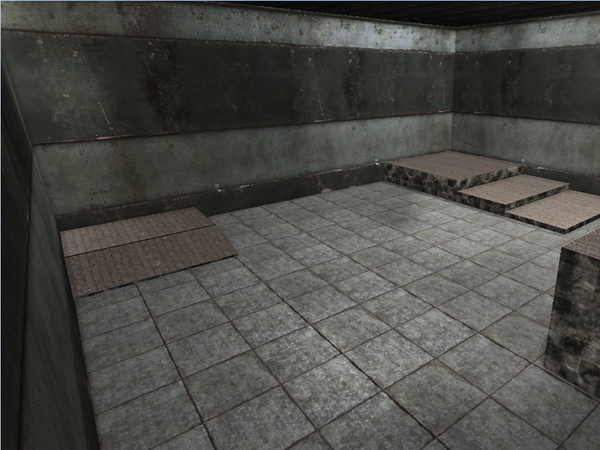
\includegraphics[width=4cm]{images/Worlds/testRoom.jpg}}\qquad
%\subfigure[Factory,]{\label{3D_World-c}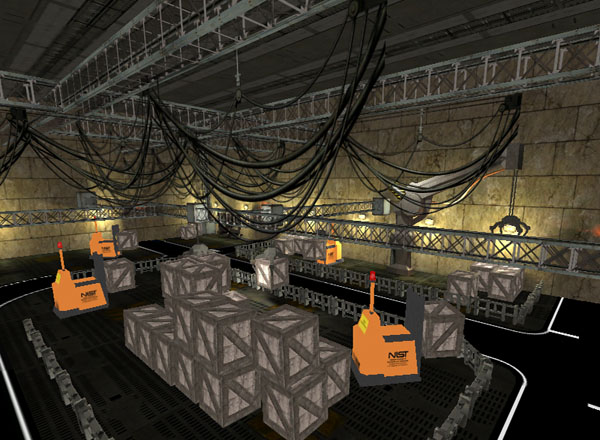
\includegraphics[width=4cm]{images/Worlds/factory.jpg}}
%\caption{Sample of 3D environments in USARSim.} \label{3D_World}
%\end{figure}
%\begin{figure}[t!]
%\centering
%\subfigure[Air Robot AR100B.]{\label{Fig:AirRobot}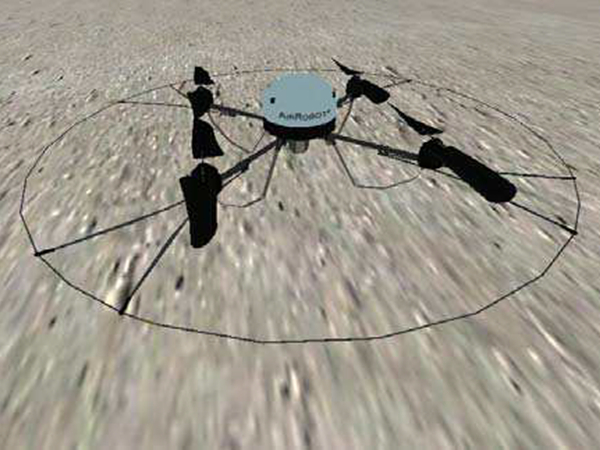
\includegraphics[width=4cm]{images/Robots/airRobot_2.jpg}}\qquad
%\subfigure[Kuka KR60,]{\label{Fig:KR60}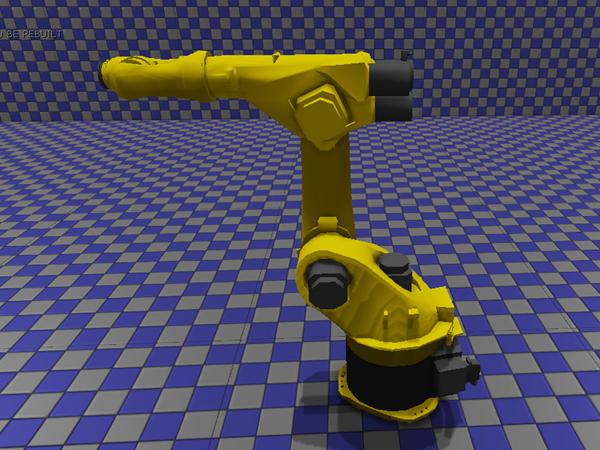
\includegraphics[width=4cm]{images/Robots/kr60.jpg}}
%\caption{Sample of vehicles in USARSim.}
%\end{figure}
%USARSim was initially developed with a focus on differential drive wheeled robots. However, USARSim's open source framework has encouraged wide community interest and support that now allows USARSim to offer multiple robots, including humanoid robots, aerial platforms (Figure~\ref{Fig:AirRobot}), robotic arms (Figure~\ref{Fig:KR60}), and commercial vehicles. All robots in USARSim have a chassis, and may contain multiple wheels, sensors, and
%actuators. The robots are configurable (e.g. specify types of
%sensors/end effectors) through a configuration file that is read at run-time. The properties of the robots can
%also be configured, such as the battery life and the frequency of
%data transmission.

%%--------------
USARSim was originally based upon simulated environments in the (Urban Search and Rescue) USAR domain. Realistic disaster scenarios as well as robot test methods were created (Figure~\ref{TestRoom}).
Since then, USARSim has been used worldwide and more environments have been developed for different purposes. Other environments such as the NIST campus (Figure~\ref{3D_World-b}) and factories (Figure~\ref{3D_World-c}) have been used to test the performance of algorithms in different efforts~\cite{WANG.HFES.2005,BALAGUER.IROS.2008,KOOTBALLY.ITEA.2010}. The simulation is also widely used for the RoboCup Virtual Robot Rescue Competition \cite{RoboCupWeb}, the IEEE Virtual Manufacturing and Automation Challenge \cite{VMACWeb}, and has been applied to the DARPA Urban Challenge (Figure~\ref{3D_World-a}).

\begin{figure}[t!]
\centering
\subfigure[Test Room.]{\label{TestRoom}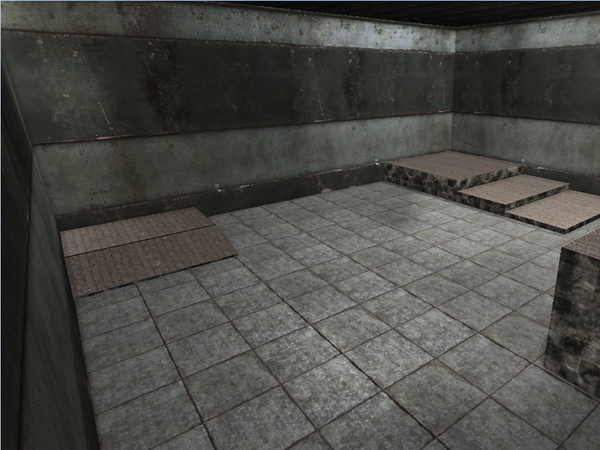
\includegraphics[width=4cm]{images/Worlds/testRoom.jpg}}\qquad
\subfigure[NIST main campus.]{\label{3D_World-b}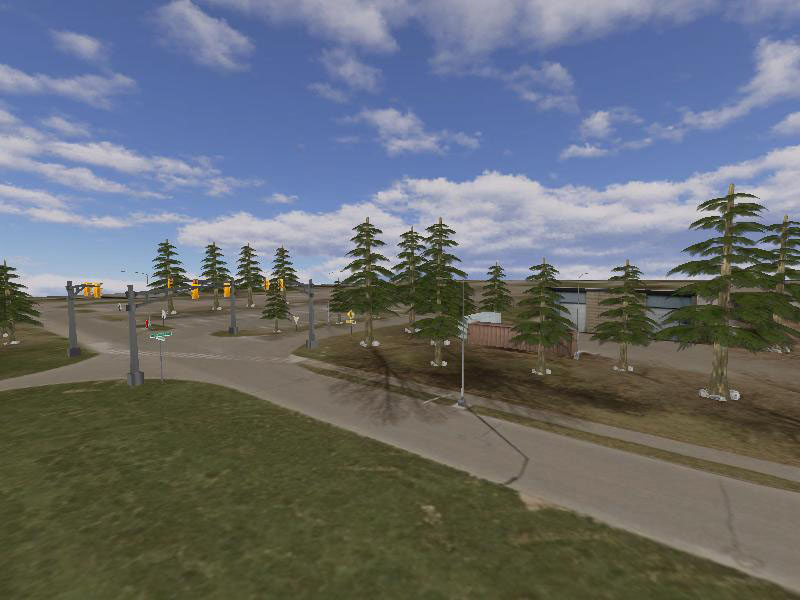
\includegraphics[width=4cm]{images/Worlds/nist2.jpg}}\qquad
\subfigure[Factory,]{\label{3D_World-c}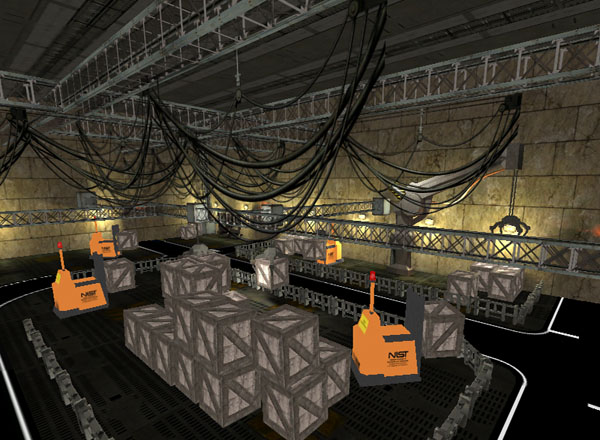
\includegraphics[width=4cm]{images/Worlds/factory.jpg}}\qquad%
\subfigure[Road course.]{\label{3D_World-a}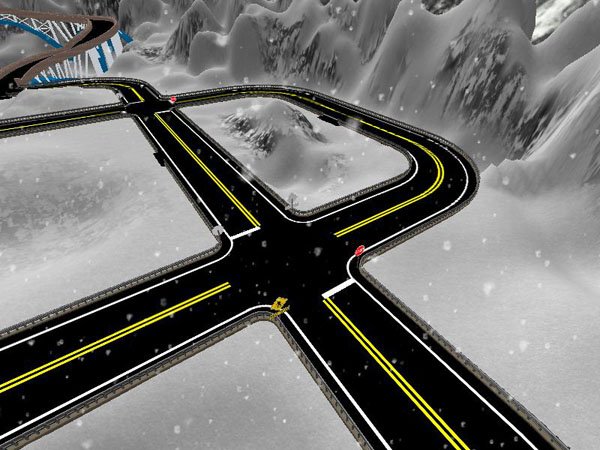
\includegraphics[width=4cm]{images/Worlds/arda1.jpg}}
\caption{Sample of 3D environments in USARSim.} \label{3D_World}
\end{figure}

USARSim was initially developed with a focus on differential drive wheeled robots. However, USARSim's open source framework has encouraged wide community interest and support that now allows USARSim to offer multiple robots, including humanoid robots (Figure~\ref{Fig:Nao}), aerial platforms (Figure~\ref{Fig:AirRobot}), robotic arms (Figure~\ref{Fig:KR60}), and commercial vehicles (Figure~\ref{Fig:Kiva}). In USARSim, robots are based on physical computer aided design (CAD) models of the real
robots and are implemented by specialization of specific existing classes. This structure allows for easier development of new platforms that model custom designs.

All robots in USARSim have a chassis, and may contain multiple wheels, sensors, and
actuators. The robots are configurable (e.g., specify types of
sensors/end effectors) through a configuration file that is read at run-time. The properties of the robots can
also be configured, such as the battery life and the frequency of
data transmission.

\begin{figure}[t!]
\centering
\subfigure[Aldebaran Robotics Nao.]{\label{Fig:Nao}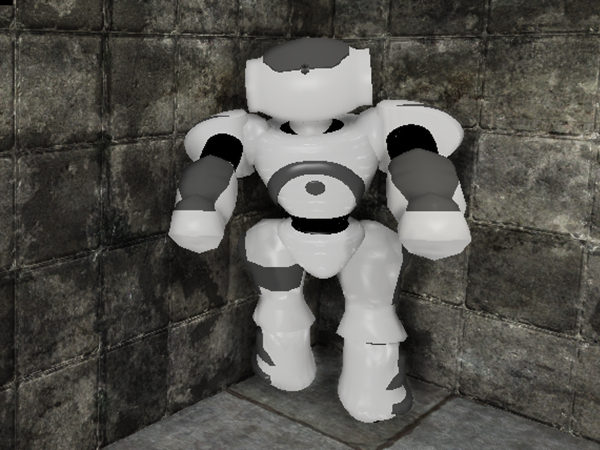
\includegraphics[width=4cm]{images/Robots/nao.jpg}}\qquad
\subfigure[Air Robot AR100B.]{\label{Fig:AirRobot}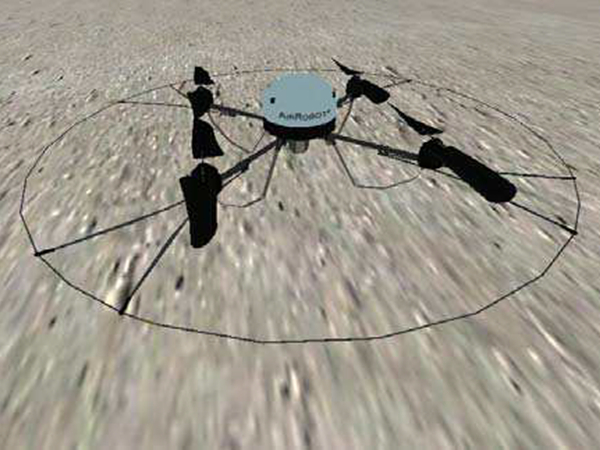
\includegraphics[width=4cm]{images/Robots/airRobot_2.jpg}}\qquad
\subfigure[Kuka KR60,]{\label{Fig:KR60}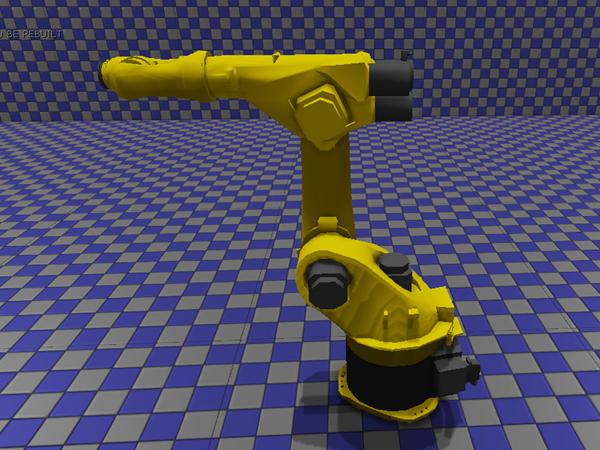
\includegraphics[width=4cm]{images/Robots/kr60.jpg}}\qquad
\subfigure[Kiva Robot.]{\label{Fig:Kiva}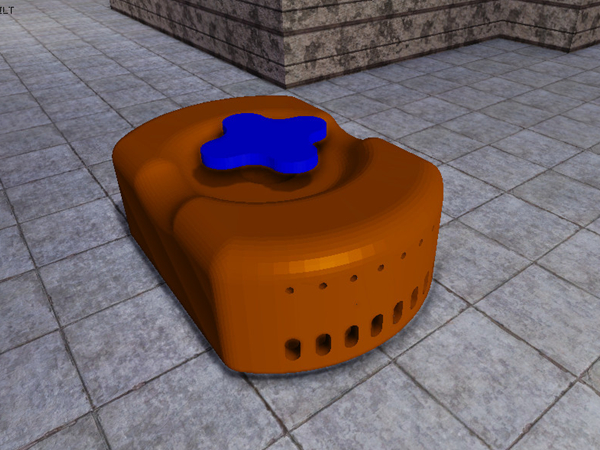
\includegraphics[width=4cm]{images/Robots/kiva.jpg}}
\caption{Sample of vehicles in USARSim.}
\end{figure}

\subsection{The Simulated Sensor System}
\label{subsection:usartruth}
Poses of objects in the virtual environment are retrieved with the USARTruth tool. USARTruth is capable of reading information about objects in USARSim by connecting as a client to TCP socket port 3989. The simulator USARTruthConnection object listens for incoming connections on port 3989 and receives queries over a socket in the form of strings formatted into key-value pairs.

The USARTruth connection accepts two different keys, ``class'' and ``name''. When USARSim receives a new string over the connection, it sends a sequence of key-value formatted strings back over the socket, one for each Unreal Engine Actor object that matches the requested class and object names. An example of the strings returned by USARSim is given below along with a description for each key.


\{Name P3AT\_0\} \{Class P3AT\} \{Time 29.97\} \{Location 0.67,2.30,1.86\} \\ \{Rotation 0.00,0.46,0.00\} where:
%\{Name P3AT\_0\} \{Class P3AT\} \{Time 29.97\} \{Location 0.67,2.30,1.86\} \{Rotation 0.00,0.46,0.00\} where:
%The return strings include the following keys:

\begin{itemize}
\item Name: The internal name of the object in USARSim.
\item Class: The name of the most specific Unreal Engine class the object belongs to.
\item Time: The number of seconds that have elapsed since the simulator started, as a floating-point value.
\item Location: The comma-separated position of the object in global coordinates.
\item Rotation: The comma-separated orientation of the object in global coordinates, in roll, pitch, yaw form.
\end{itemize}


%The virtual sensor system uses USARTruth to simulate real-world sensors by opening a new USARTruth connection and sending one request for specified Unreal Engine class names.

% each different Unreal Engine class name found in the \textsf{MySQL Database}. For simulation purposes, the Unreal Engine class name is stored as an object's ``external shape''. It is important to note that the Location and Rotation values coming out of USARTruth do not include noises and assume perfect sensor data.
%
% The system then parses the data coming in from USARTruth and updates the relative pose in the MySQL database for each object returned. Since USARTruth returns object locations in global coordinates, the relative pose for each object is updated without changing its transformation tree; that is, the RefObject for its PhysicalLocation is unchanged. The actual updated relative pose is computed according to
% \begin{equation}
% L' = LG^{-1}G'
% \end{equation}
% where $L'$ is the updated relative transformation, $L$ is the old relative transformation (read from the MySQL database), $G$ is the old global transformation (computed from the transformation tree in the database), and $G'$ is the updated global transformation (retrieved from USARTruth).


%\section{Example of Operation}
\label{sec:sensor}

\subsection{TODO}
\begin{itemize}
\item Describe the interaction between the predicate evaluation and the update of the MySQL database from sensor data.
\item Describe in more details the work that Teddy did to query the sensor
\end{itemize}

%USARTruth~\cite{} comes with the USARSim framework. USARTruth is capable of reading out information on objects in USARSim by connecting as a client to TCP socket port 3989 and sending a message indicating the type of object the user is interested in.

USARSim can be directly queried to return the 6DOF pose of a specific object, or of every object of a certain type. The simulator USARTruthConnection object listens for incoming connections on port 3989, and receives queries over a socket in the form of strings formatted into key-value pairs. The USARTruth connection accepts two different keys, ``class'' and ``name,'' which are both optional. When USARSim receives a new string over the connection, it sends a sequence of key-value formatted strings back over the socket, one for each Unreal Engine Actor object that matches the requested class and object names. The return strings include the following keys:

\begin{itemize}
\item Name: The internal name of the object in USARSim.
\item Class: The name of the most specific Unreal Engine class the object belongs to.
\item Time: The number of seconds that have elapsed since the simulator start, as a floating-point value.
\item Location: The comma-separated position of the object in global coordinates.
\item Rotation: The comma-separated orientation of the object in global coordinates, in roll, pitch, yaw form.
\end{itemize}

The virtual sensor system uses USARTruth to simulate real-world sensors by opening a new USARTruth connection and sending one request for each different Unreal Engine class name found in the MySQL database. For simulation purposes, the Unreal Engine class name is stored as an object's ``external shape.''

The system then parses the data coming in from USARTruth and updates the relative pose in the MySQL database for each object returned. Since USARTruth returns object locations in global coordinates, the relative pose for each object is updated without changing its transformation tree; that is, the RefObject for its PhysicalLocation is unchanged. The actual updated relative pose is computed according to
\begin{equation}
L' = LG^{-1}G'
\end{equation}
where $L'$ is the updated relative transformation, $L$ is the old relative transformation (read from the MySQL database), $G$ is the old global transformation (computed from the transformation tree in the database), and $G'$ is the updated global transformation (retrieved from USARTruth).
%---------------------------%
\section{System Operation}\label{section:sensor}
\section{Example of Operation}
\label{sec:sensor}

\subsection{TODO}
\begin{itemize}
\item Describe the interaction between the predicate evaluation and the update of the MySQL database from sensor data.
\item Describe in more details the work that Teddy did to query the sensor
\end{itemize}

%USARTruth~\cite{} comes with the USARSim framework. USARTruth is capable of reading out information on objects in USARSim by connecting as a client to TCP socket port 3989 and sending a message indicating the type of object the user is interested in.

USARSim can be directly queried to return the 6DOF pose of a specific object, or of every object of a certain type. The simulator USARTruthConnection object listens for incoming connections on port 3989, and receives queries over a socket in the form of strings formatted into key-value pairs. The USARTruth connection accepts two different keys, ``class'' and ``name,'' which are both optional. When USARSim receives a new string over the connection, it sends a sequence of key-value formatted strings back over the socket, one for each Unreal Engine Actor object that matches the requested class and object names. The return strings include the following keys:

\begin{itemize}
\item Name: The internal name of the object in USARSim.
\item Class: The name of the most specific Unreal Engine class the object belongs to.
\item Time: The number of seconds that have elapsed since the simulator start, as a floating-point value.
\item Location: The comma-separated position of the object in global coordinates.
\item Rotation: The comma-separated orientation of the object in global coordinates, in roll, pitch, yaw form.
\end{itemize}

The virtual sensor system uses USARTruth to simulate real-world sensors by opening a new USARTruth connection and sending one request for each different Unreal Engine class name found in the MySQL database. For simulation purposes, the Unreal Engine class name is stored as an object's ``external shape.''

The system then parses the data coming in from USARTruth and updates the relative pose in the MySQL database for each object returned. Since USARTruth returns object locations in global coordinates, the relative pose for each object is updated without changing its transformation tree; that is, the RefObject for its PhysicalLocation is unchanged. The actual updated relative pose is computed according to
\begin{equation}
L' = LG^{-1}G'
\end{equation}
where $L'$ is the updated relative transformation, $L$ is the old relative transformation (read from the MySQL database), $G$ is the old global transformation (computed from the transformation tree in the database), and $G'$ is the updated global transformation (retrieved from USARTruth).

%---------------------------%
\section{Conclusions and Future Work}\label{section:conclusions}
\section{Conclusions and Future Work}
\label{sect:future}
The framework described in this paper has been applied to the domain of kit building, which is a simple, but practically useful manufacturing/assembly domain. Through its use, we have been able to demonstrate agility in both kit construction through late binding of part locations, and in recovery from action failures through the detection of failures and ability to compensate for the failure's effects.

There are several areas in the system that still utilize hand-coding of data. It is desired that extensions to the ontology be created that will allow for the automatic application of knowledge and eliminate code that it specifically tuned to a particular set of predicates or actions. The hand-coded areas include the conversion of PDDL actions to CRCL sequences as well as the retrieval of instance data from the MySQL database for predicate evaluation. Work is currently underway to correct for these deficiencies. 

Extensions are also possible that will expand this work to the realm of general assembly. We hope to apply this knowledge based framework to simple assembly tasks (growing towards more complex tasks) on a real robot workcell in the near future. 


%---------------------------%
\section{NIST Disclaimer}
This publication was prepared by a Guest Researcher with the United States Government, was funded in part through Government support, and is, therefore, a work of the U.S. Government and not subject to copyright.

%---------------------------%
\section{Acknowledgement}
The authors would like to extend our gratitude to Grayson Moses, who worked at NIST as a Poolesville High School student volunteer and helped with the development of algorithms to task a sensor system to provide updated pose information.
%
% ---- Bibliography ----
%
\bibliographystyle{plain}
\bibliography{rita2013}
\clearpage
\addtocmark[2]{Author Index} % additional numbered TOC entry
\renewcommand{\indexname}{Author Index}
\printindex
\clearpage
\addtocmark[2]{Subject Index} % additional numbered TOC entry
\markboth{Subject Index}{Subject Index}
\renewcommand{\indexname}{Subject Index}
%\input{subjidx.ind}
\end{document}
